%!TEX root = ../thesis.tex

\cleardoublepage
\chapter{Approach}
\label{cha:approach}

To discuss the solution implemented for this thesis requires a review of, firstly, the requirements contained in the problem statement, and, secondly, a description of both the decisions made as well as the process behind making those decisions. To that extent, this chapter will discuss, the components needed in order to address the problem statement. It will try to discuss not only what decisions were made, but also, crucially, what decisions were \textit{not} made, and why. The first section will begin with the fundamental nature of the solution's architecture, thereafter a review of the design requirements which arise from the Deterministic Networking specification will follow, finally the precise nature of the solution's internal workings will be presented.

\section{Requirements}

Concretely, a multipath backhaul solution, as has been described in the introduction, will need to be able to transport the 5G traffic from the edge deployment to the core, while respecting the traffic's QoS requirements. This breaks down into a short list of hard requirements.

\begin{enumerate}
  \item Forward only the appropriate traffic (as is defined in the 5G flow descriptions)
  \item Manage multiple outgoing paths
  \item Co-ordinate flows and their requirements with the Control Plane
  \item Select the best path to enable the flow's requirements and achieve determinism
\end{enumerate} 

%%=========================================
\section{Skeleton Structure}
\label{sec:approach:plan}

At the outset of this thesis it was decided to use a Control User Plane split. The packet processing and forwarding is performed in the user plane, and the control plane makes the high level decisions about which packets to send where, and in this case, on which outgoing interface to send them. The data plane is kept simple and only performs the time critical packet processing, and blindly follows the instructions of the control plane. This type of architecture is very common in modern software-based networks, for example OpenFlow, the Evolved Packet Core (from LTE), and the 5G core all implement this kind of Control-Data-Plane split.

However, this decision immediately locks one into certain positions. For example, this requires a method of communication between the data plane and the control plane, it also means the state machine that represents the WAN Connector becomes more complex, and complexity always brings with it a greater danger for hidden mistakes and fallacies. The benefit is that the user plane function does not need to perform any of its own decisions, thus simplifying its internal architecture, and these components can be deployed at different locations, and scaled up or out with greater ease.

%%=========================================
\section{Architectural Components Required for Deterministic Multipath Backhaul in a 5G Campus Environment}
\label{sec:approach:req}

Determinism, in a networking context, refers to the ability of a network to supply specific QoS requirements with extremely high degrees of certainty. IP flows and applications running in these networks are assured they will experience bounded latency, jitter, and packet loss. To this extent, the Determinsitic Networking specification (also called DetNet) is a specification with recommendations for how to achieve determinism. However it does not define determinism. A network which does not fully comply to these specifications may still call itself determinstic (but it may not say it is a DetNet). Since this thesis aims to provide determinstic backhaul, it is not required to follow the DetNet specifications in any form. Though, it does make sense to consider what solutions they have proposed for determinism, since ultimately the goals are the same. In this section, therefore, the DetNet specifications will be used as a source of inspiration to gleam ideas, but not as an absolute source of truth.

Deterministic networks have been discussed in the previous chapter. In order to guarantee determinism the IETF DetNet working group has proposed an architecture for determinism over IP networks \cite{finn2019deterministicArch}. Their specification identifies four key mechanisms for guaranteeing the determinism of a flow: 1) elimination of contention loss, 2) jitter reduction, 3) service protection, and 4) explicit routes. Since the 5G campus environment may need to use the infrastructure of other operators this rules out the ability to use explicit routes. A key difference between deterministic networks and 5G campus backhaul networks is that the operator may not control all the links between nodes, and that there are only two nodes in the network that are definitely under the administrator's control- the WAN Connectors at the core and the edge. In such a scenario the problem is less like a network and more like a client - server application with multiple paths between the client and the server.

\subsection{Elimination of Contention Loss and Bufferbloat}

In order to prevent packet loss due to buffer overflows, and, just as importantly, to prevent high latencies due to bufferbloat \cite{gettys2011bufferbloat} or excessive queuing, contention between flows must be carefully managed. A greedy flow, which uses too much bandwidth, or the presence of too many flows, whose cumulative bandwidth demands exceed the link's capabilities, will have negative effects on all the flows running over the link.

Elimination of contention loss can be achieved by using a traffic shaper and/or rate limiter, and the ingress to any DetNet domain \textbf{must} apply such a function. For the WAN Connector therefore a traffic shaper must also be applied to the traffic on ingress, from the RAN, before it is sent across the backhaul links. Since the implementation of a traffic shaper is beyond the scope of this thesis, an existing solution must be used. The traffic control subsystem in the linux kernel (TC) provides several implementations of different algorithms for both rate limiting and traffic shaping. Some of these algorithms have already been discussed in the previous section. For the purposes of this solution several algorithms were considered: Hierarchical Token Bucket (HTB), Hierarchical Fair Service Curve (HFSC) \cite{stoica1997hierarchical}, Time Aware Prioriy Queueing (taprio), Common Applications Kept Enhanced (CAKE) \cite{hoiland2018piece}, and Fair Queuing with Controlled Delay (FQ\_CoDel).

For HTB and HFSC, due to the implementation of these algorithms in the linux tc subsystem, integrating them within the context of this solution would require filters for each flow. This is not necessarily a hindrance yet, however it would introduce additional overhead upon the creation and/or addition of each new flow. Perhaps more importantly, the implementation of the HTB algorithm provides no means for fair queuing. This means that while it is not possible for greedy and/or malicious flows to use up the bandwidth of other flows because HTB guarantees bandwidth, the greedy flows can cause other flows to experience higher latency because it does not guarantee delay. The HFSC algorithm improves on this by offering both bandwidth and delay guarantees. However this makes it far more difficult to configure, and would require precise calculation of the service curve for each new flow.

Another feasible option available in linux TC would be the time aware priority queuing (taprio). This queuing discipline provides scheduled gates for specific traffic classes. It could be used to schedule flows according to their requirements and/or priorities, and thus provide a form of prioritization, and, to an extent, traffic shaping. Flows can be assigned different windows and congestion due to a greedy flow is avoided if it is scheduled for a different window. However one issue is that taprio fails to provide fair queuing, and thus would need to be configured and possibly adapted as new flows are added and removed, depending on their priority. Greedy flows of the same priority would have to fight each other to use the bandwidth available in their assigned window.

Lastly there are FQ\_CoDel and CAKE. Both provide fair queuing as well as active queue management, which means flows are less likely to experience loss due to congestion, particularly congestion caused by one particularly greedy flow. Since the CAKE algorithm was originally designed for routers in WLAN networks, and these are loosely analogous to a 5G campus network (consider the User Equipment as the Stations, and the Base Station as the Access Point), it makes it an attractive choice. CAKE also allows the use of 8 different priority tins, which fits well with the nature of 5G traffic, where different flows have different priorities. Finally, on a practical level, the implementation of CAKE in the linux kernel uses the kernel's "skb\_flow\_dissector" which exposes a hook point for eBPF \footnote{https://www.kernel.org/doc/html/v5.1/networking/bpf\_flow\_dissector.html\#overview} programs. Specifically within a 5G context, this could allow one to attach an eBPF program to allow CAKE to peek inside of GTP tunnels, and differentiate the flows within them. For all the other algorithms mentioned so far, all of the GTP packets would appear to belong to the same flow, and thus none of these algorithms would work at all if the traffic is arriving in a GTP tunnel. This is ultimately the strongest case that can be made for any of the options listed so far. TC does have one other algorithm which hooks into the "skb\_flow\_dissector", namely the Choose and Keep Scheduler (CHOKe) \cite{pan2000choke}, which does perform active queue management, however does not provide fair queuing. This means that while it manages buffers in order to prevent them from filling up, it does not guarantee different flows a fair share of the bandwidth, which can still lead to flows experiencing increased delay due to other greedy flows.

\subsection{Jitter Reduction and Latency Guarantees}

In the Deterministic Networking Architecture specification it is recommended to adopt time synchronization as well as sending "Time of Execution" fields in the application packets, in order to achieve jitter reduction. For time synchronization, the PTP protocol may serve well, especially since there is an existing implementation- the linuxptp project -  which extends it to work over IP networks. As for the time of execution fields, it may be possible to place these in a GTP header, or to combine them with timestamping.

Latency guarantees are not mentioned within the specification but they are important for the 5G campus setting. Specifically when backhaul options may include satellite links it becomes important to consider latencies. Additionally, in a multipath setting, latency can be a useful criteria for selecting between links, and guaranteeing latency becomes easier to do when it is possible to switch links should one of them start to experience greater latency than before.

\subsection{Service Protection}

In order to protect against equipment failure, it may be recommendable to perform packet replication and/or encoding. To address this the DetNet specification speaks of both duplication of flows, and network coding \cite{ahlswede2000network}. This can be a clever solution, however Network Coding requires control over and co-ordination between all the nodes in the network (like other parts of the Deterministic Networking specifications). Though to guard against equipment failure and/or packet loss, duplication does provide an option. So too, does forward error correction (FEC). Many FEC schemes work on a continuous stream of bytes, providing correction for bit errors, as opposed to correcting the loss of entire packets. There are schemes which address this, fountain codes - such as Raptor \cite{luby2007raptor}, which encode the data as being made up of multiple discrete symbols, and these symbols can be mapped directly to packets, thus allowing the Raptor FEC algorithm to protect against packet loss as opposed to just bit erros. Unfortunately the open source ecosystem surrounding fountain codes is not as developed as that around other FEC schemes, and, because of the complexity involved in implementing them efficiently, there are relatively few freely available projects or libraries which can be used to encode packets using such a scheme. For reference, \footnote{https://aff3ct.github.io/fec\_libraries.html} mainaints a list of C/C++ FEC libraries and none of them support the Raptor family of fountain codes (all other fountain codes incur high overhead). Even if it were more feasible to integrate FEC into the backhaul solution it bears questioning how much benefit it brings. FEC is very powerful in situations with consistently lossy links, however paths over the internet tend to experience loss in bursts, as opposed to at a consistent rate. To this extent it may make more sense to duplicate those flows which require a high degree of reliability. 

%Flow duplication will mean a packet ordering and elimination function will be required, to eliminate those packets which arrive twice, and to re-order other ones.

If one does choose to duplicate packets in order to achieve service protection, that means an elimination function is also required, as well as a packet ordering function. This is because multiple packets may arrive on one link before they arrive on the backup path. If a packet got lost on the faster path, it may still show up on the slower one and thus the packet forwarding needs to pause until the missing packet arrives. The DetNet specifications provide both a basic and an advanced Packet Ordering Function (POF) algorithm. This algorithm can be very easily adjusted to also perform the elimination of duplicate packets. The DetNet specification also clarifies how long one should wait to see if the missing packet arrives (or doesn't) - this value "cannot be smaller than the delay difference of the paths used by the flow" and is called the $POFMaxDelay$.

\begin{algorithm}[H]
\label{pof-alg}

\tcc{initialization}
\lForEach {flow $f$}{$POFLastSent_f \leftarrow 0$}
\tcc{Start POF logic}
\While{true}{
receive packet $p$, with sequence number $seq\_num$ for flow $f$\;

\eIf{$seq\_num <= POFLastSent_f + 1$}{
\tcc{eliminate duplicates}
\If{$seq_num == POFLastSent_f +1$}{
forward $p$\;
$POFLastSent_f = seq\_num$\;
}
}{
\tcc{in a separate thread}
buffer $p$ until $seq\_num = POFLastSent_f + 1$ \textbf{or} $POFMaxDelay_f$ elapses\;
forward $p$\;
$POFLastSent_f = seq\_num$\;
}
}

\caption{Basic POF Algorithm Adjusted for De-Duplication}
\end{algorithm}

The algorithm shown in \ref{pof-alg} is the Basic POF algorithm, with a single adjustment made on line 5 to make sure that an incoming packet's sequence number is not lower than the next one we are expecting, in order to properly eliminate duplicates. The algorithm's \textbf{if/else} logic in this representation could be unified in a cleaner way, but it was done this way specifically because it thus requires just one extra line (line 5) to be changed from the DetNet specifications POF algorithm, and that one change suffices to make it a Packet Ordering and Elimination Function.

\subsection{Multipath Considerations}

While the previous subsections have all considered requirements for determinism in an IP network, the issue of multipathing still remains. For a component which is backhauling over multiple links in an IP networks this means link and/or path selection is required. Traditionally, routers select links primarily based on their ability to route the packet to the destination, and secondarily based on various metrics, which can be defined by the administrator. For the WAN Connector's scenario routing considerations are not made- it's purpose is to backhaul the traffic from the RAN / Edge to the Core, where the network's own internet gateway can perform the routing.

At this point it is crucial to differentiate, again, between multihoming and multipathing. Multihomed hosts are able to select one of many links for their outgoing traffic's destination. In multipathing the same link may lead to multiple paths to \textit{different} destinations. When two multihomed hosts communicate with eachother multiple different paths are opened up. Multipathing over the internet requires complex data collection about all the routers in between the source and the destination, see \cite{ganichev2010yamr} for an example of such an implementation. This is because multipathing over the internet needs to choose paths with maximally edge-disjoint paths to achieve the best reliability, as well as maximally vertex-disjoint paths in order to reduce the load across all nodes on the path.

The goal of this thesis is of course to use the link and/or path selection to provide determinism for the flows being backhauled. To this extent then, the link selection algorithm must attempt to forward flows over paths which can provide at worst the maximum allowed latency and jitter, as well as meeting the minimum reliability. Here it is worth noting that while duplication cannot really be used to guarantee latency, it can be used to improve reliability since a flow which is duplicated across two paths is far less likely to experience packet loss.

\subsection{Summary of Necessary Features}


Looking back on the previous subsections, the following points (in no particular order of priority) were identified as mandatory for a deterministic backhaul solution: 1) traffic shaping, 2) path selection according to jitter and latency requirements, 3) service protection (i.e. via packet duplication), 4) packet ordering and de-duplication, and 5) time synchronization. The ways in which these can be addressed, or quite simply the way in which they were implemented, will be discussed in the following section

%%=========================================
\section{Overview of the WAN Connector's Features and Components}
\label{sec:approach:arch}

At this point, one can take the skeleton structure proposed in the first section, and superimpose the other requirements which were determined in the second section. Combining these ideas yielded the final implementation, which will be now be presented.

\subsection{Path Selection Algorithm}

Meeting the various requirements - jitter, latency, and delay - of a flow can be formulated as a multi-constrained QoS problem. Solving such a multi-constrained QoS problem via path selection is a binary optimization problem, and the key to deterministically meeting the flows requirements. The problem can be posed as: "select those paths on which to forward packets while making sure to satisfy the latency, jitter and reliability requirements of the given flow, and minimizing the overall weight of the paths used". The mathematical definition is as follows:

\begin{gather}
\label{algorithm}
\text{Minimize } \sum_{i=1}^{P}w(x_i) \\
\text{Where,   } d(i) * x_i\le D \\
j(i) * x_i \le J \\
1 - \prod_{i=1}^{P}{ ( 1- r(i) * x_i ) } \ge R  \\
\text{for } x_i \in \{0,1\}
\end{gather}

Here the variables $D$, $J$, and $R$ are the flow's delay, jitter, and reliability requirements, while the functions $d(i)$, $j(i)$, $r(i)$, $w(i)$ are the estimated delay, jitter, reliability, and weight of link $i$. The predicted values will usually just be the latest measurement, as recommended in \cite{akella2008performance}, however there is room here to use more advanced metrics to predict the future link quality and thus perform preemptive path switching in future work. The total number of paths is $P$. The $x_i$ variable indicates whether or not link $i$ shall be used. If a solution is found, then the flow's packets will be forwarded on each link $i$ where $x_i = 1$, and if no solution can be found which satisfies these conditions then the flow is rejected because its QoS cannot be guaranteed.

It is worth noting that solving such problems is NP-Hard \cite{ilp-np-hard}. However this hardness arises primarily because of equation 3.4, the equation for reliability (also the only non-linear equation). Due to this equation one must consider every possible combination of paths on which to forward, and the complexity is $O(2^n)$. This means, even though akella et. al \cite{akella2003measurement} have shown that multihomed approaches experience diminishing returns after more than 4 links, attempting to brute force the solution by limiting the number of outgoing interfaces to 4 still yields a very large problem space - in the worst case both WAN connectors could have 4 outgoing paths, leading to 16 possible paths and thus 65536 possible combinations to consider.

In order to further avoid the combinatorial explosion the problem needs to be parameterized even more. The first logical parameterization has already taken place by limiting the number of interfaces to 4. This can be expanded on by limiting duplication to only take place over disjoint interfaces. The reasoning behind this is that in a geographically distributed Campus 5G environment, and especially for environments featuring wireless backhaul (e.g. satellite), it is more likely that a link's reliability is most affected by the over the air transmission on the first hop. By performing this parameterization the problem space shrinks considerably, to just $2^4$ possible combinations of outgoing paths, but, because certain paths going out on the same interface are ignored, the optimality of the overall solution is gone. This is an acceptable trade off for quick computation, and reasonably strong guarantees on reliability. When choosing which path to include from a set of paths using the same outgoing link, only the path with the greatest reliability is taken into consideration so that the likelihood of rejecting a potentially viable flow is as low as possible.

\subsection{Packet Ordering and Elimination Function}

Since it is possible for flows to be duplicated across multiple paths, it becomes a necessity to have a packet ordering and elimination function. To be able to re-order and de-duplicate packets means that their sequence numbers need to be tracked. This thesis' implementation will track the sequence number on a per flow basis, using the GTP "sequence number" field. This thesis uses it's variation of the DetNet POF specification's Basic POF algorithm \cite{ietf-detnet-pof-08}, as presented in \ref{pof-alg}.

\subsection{Internal Architecture}

\subsubsection{Control - Data Plane Communication}

A protocol is desired which can provide reliable communication over multiple paths in order to communicate between the data plane and the control plane which is where the statistics are collected, flows are added or removed, and the multipath decisions are made. This is crucial, since in a geographically distributed campus 5G deployment it is unlikely that there will be a separate management or control network which uses different underlying network infrastructure than the data plane. Therefore link failure, as well as packet loss, on the link being used by the control plane must either be avoided or protected against. To this extent there are only two feasible options - either multipath TCP or SCTP. SCTP does support multihoming and intelligent failover, despite not being explicitly designed for multipathing, and is slightly easier to manage and configure than multipath TCP, which is why it was chosen for the data plane control plane interactions.

\subsubsection{GTP Tunneling and Custom Header Extension}

The tunneling protocol used between the two data plane instances of the WAN Connector will  be GTP version 1 \cite{3gpp.29.060}. The specification for GTP allows for the use of sequence numbers, as well as the use of extension headers. For the data plane communication there will always be an additional custom header sent which includes a timestamp taken by the sender. The timestamp is taken in microseconds. For the timestamp there are several options available within linux. The TAI clock in linux (representing the Atomic International Time) is used in this implementation because it does not have leap seconds, and so is a monotonic function, which is an important guarantee for time sensitive applications. An example of a packet capture of the WAN Connector using the custom header is included in the appendix \ref{appendix:gtp}.

Normally, in 64 bit linux systems, a timestamp takes up 16 bytes and consists of 8 bytes for the time in seconds since the epoch, and another 8 bytes for the nanoseconds. To reduce the footprint of the timestamp in the header, the seconds are represented with just 8 bytes, thus wrapping around the interval $[0,255]$. The receiver needs to take this into account, but is programmed to do so, and since the path delays are not realistically expected to ever exceed 3 seconds this is more than enough. The microseconds have a maximum value of $10^6$ and can be represented with just 24 bits. For Wide Area Networks and internet connections usually the latencies are on the order of milliseconds and as such microsecond precision is deemed to be sufficient.

\subsubsection{Metric Collection}

To be able to intelligently switch flows between paths, and to be able to know when this is required, it is necessary to collect the relevant metrics about latency, jitter, bandwidth usage, as well as packet loss. Packet loss can be detected via the sequence numbers, while delay and jitter can be calculated using the timestamps passed along in the GTP headers. These metrics are periodically reported to the control plane so that it can make its decisions on up to date data. Keeping a healthy overview over the state of each path requires periodic probing on these paths. This is especially important for detecting when paths become viable again, since these paths will not have any traffic on them while they are considered down, or if they have experienced high latency and/or jitter recently. The probes are sent once per period of reporting so that they have a minimal impact on the bandwidth usage.

\subsubsection{Flow Descriptions, Flows, and Hashing}

Incoming packets need to be quickly mapped to their respective flows. It is common in network environments to perform flow hashing, in order to quickly lookup which flow incoming packets belong to. This approach makes sense here too. However, since 5G flow descriptions can apply to various IP and port ranges as well as matching based on the transport layer protocol it is not possible to hash an incoming flow and obtain the same hash as the flow description. Furthermore it is possible for a flow to match multiple different flow descriptions. In these cases the first matching flow description is taken. This implies some sort of ordered storage of flow descriptions will be required, as well as a method to quickly match packets to flows. The solution used here is to maintain a simple linked list of the known flow descriptions, and match packets to their flow descriptions, if the packet is unknown. For "known" packets, which have been matched to a flow description, these are hashed and stored in a table, alongside their flow descriptor and a list of paths on which the flow is supposed to be forwarded. This allows quick lookup for every subsequent packet, as well as making it simple to change which paths flows are meant to be forwarded on. One alternative to storing the flow descriptions in a linked list would be to store them in a tree, such as in \cite{flow-lookup-trees-phd}, sorted either by priority or ID or even by the hash value of the flow description. This method would provide a faster lookup of new, "unknown" packets, whose hashes don't yet match to a flow, but since new flows are not such a frequent event the additional complexity of implementing such a data structure may not be worth the gain in performance.

It is important to make a good choice when selecting a hash function. Since the hashes used are only for the purpose of lookups it would not be recommendable to pick a hashing algorithm designed for use in cryptography. These algorithms are designed so that it is very difficult to reverse engineer the original value from the hash, and this may often make the computation of the hash more computationally intensive than when computing hash algorithms designed for looking up table entries. Lastly, for hashing algorithms it is desirable that they provide a healthy distribution, to reduce collisions. Collision reduction can also be affected by choice of hash table size- and in general it is usually recommended to use a prime number. In this implementation, the MurmurHash algorithm was chosen due to its strong performance for lookup-based hashing. Specifically, the MurmurHash3 \cite{murmurhash3} version was chosen, and since it can generate 32 or 128 bit values - the exact sizes of IPv4 and IPv6 addresses - this simplifies the hashing implementation for IP flows. When a packet comes into the WAN connector it is hashed based on it's destination address, source address, destination port, source port, and finally the transport layer protocol number. If the packet was tunneled with a GTP header, the header is removed and the hash is performed on the tunneled packet, not on the GTP packet. If the hash does not match, the packets is compared to the list of existing flow descriptions. If the flow belongs to one of these descriptions then that decision is stored in the hash table.

\subsection{Overview}

\begin{figure}[h]
    \centering
        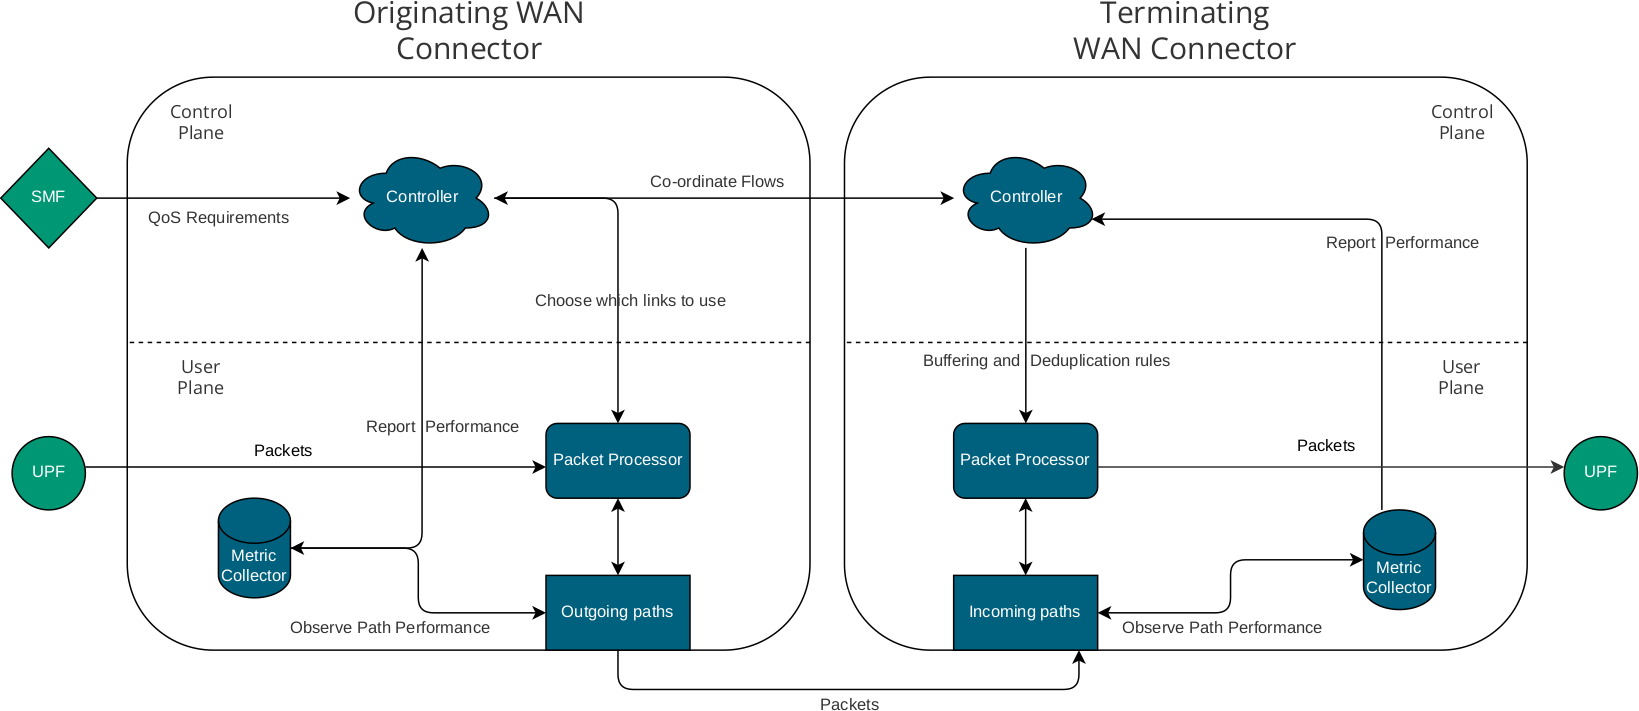
\includegraphics[width=\textwidth]{fig/be-architecture.png}
        \caption{Internal Architecture of the WAN Connector}
        \label{fig:arch}
\end{figure}

The internal architecture of the WAN connector is shown in Figure \ref{fig:arch}. The connector is split into a control plane, which uses the algorithm in \ref{pof-alg} to choose which interfaces to forward on, and a data plane, which performs the forwarding, as well as any necessary buffering, re-ordering and/or de-duplication. The WAN connector also performs different tasks depending on whether it is the origin or termination of a flow. For example, the terminating node may be receiving duplicate packets on the other paths, and it must know to drop these. Additionally, the sender, can only store statistics about how many bytes it has sent, and on what paths. The receiver is able to use the information contained in the packets it has received to construct a complete picture about the nature of the path - its jitter, latency and packet loss. The link selector in the control plane can then use this information to make its decisions.

One part which is missing from this diagram is the traffic shaper. That is because it is not connected to the control and the data plane, rather it is meant to be installed alongside them. Furthermore, it is important that the traffic shaper resides in the part of the network before the packets enter the WAN connector. If the deployment features a UPF in the edge network, it may make sense to place the traffic shaper before this as well. For the core, the traffic shaper will similarly need to be placed at the ingress point at which packets reach the WAN connector.






























